\chapter{To verify truth table for NOT gate}
%\ref{sec:background}.

%\section{Aim}
%\label{sec:objectives}
%	To verify the truth table for AND Gate.

\section{Apparatus}
%\label{sec:objectives}
	\begin{itemize}
		\tightlist
		\item Kit for realization of gates
		\item Connecting Leads
	\end{itemize}

\section{Theory}
	The NOT gate is an electronic circuit that produces an inverted version of the input at its output. It is also known as an inverter. If the input variable is A, the inverted output is known as NOT A. This is also shown as A' or A with a bar over the top, as shown at the outputs.
	\begin{figure}[h]
		\centering
		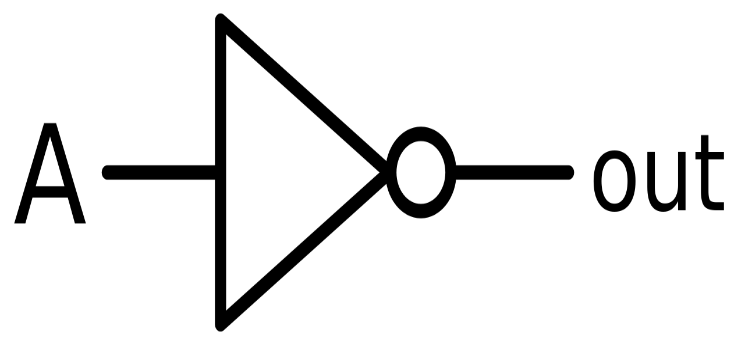
\includegraphics{img/exp3/1}
		\caption{Symbol for NOT gate}
		\label{fig:3:1}
	\end{figure}
	\begin{figure}[h]
		\centering
		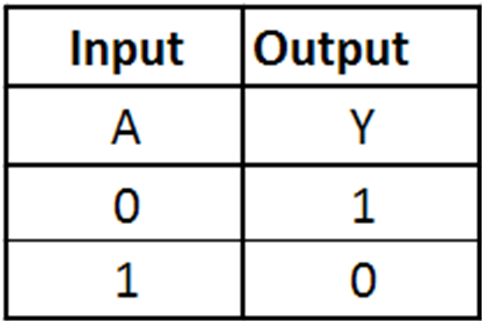
\includegraphics{img/exp3/2}
		\caption{Truth Table for NOT gate}
		\label{fig:3:2}
	\end{figure}
	NOT gate can be realized through transistor.The input is connected through resistor R2 to the transistor’s base. When no voltage is present on the input, the transistor turns off. When the transistor is off, no current flows through the collector-emitter path. Thus, current from the supply voltage (Vcc) flows through resistor R1 to the output. In this way, the circuit’s output is high when its input is low.
	
	When voltage is present at the input, the transistor turns on, allowing current to flow through the collector-emitter circuit directly to ground. This ground path creates a shortcut that bypasses the output, which causes the output to go low.
	
	In this way, the output is high when the input is low and low when the input is high.
			
	\begin{figure}[h]
		\centering
		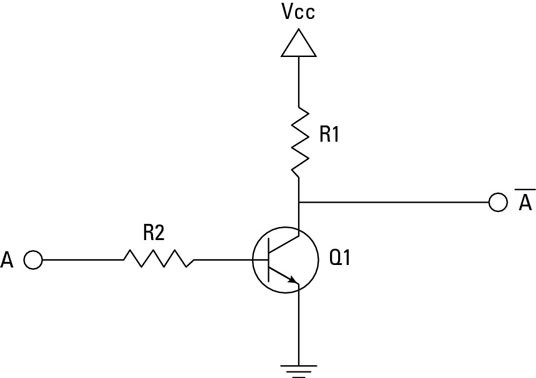
\includegraphics[width=0.3\linewidth]{img/exp3/3}
		\caption{Circut for making NOT gate}
		\label{fig:3:3}
	\end{figure}
			
\section{Procedure}
	\subsubsection{Simulator 1}
	\begin{itemize}
		\tightlist
		\item Connect the supply(+5V) to the circuit.
		\item Press the switches for inputs "A".
		\item Press the switch 2 for input "A".
		\item Repeat step-2 and step-3 for all state of inputs.
	\end{itemize}

	\subsubsection{Simulator 2}
	\begin{itemize}
		\tightlist
		\item Enter the Boolean input "A".
		\item Enter the Boolean output for your corresponding inputs.
		\item Click on "Check" Button to verify your output.
		\item Click "Print" if you want to get print out of Truth Table.
	\end{itemize}


\section{Observations}
	\begin{figure}[h]
		\centering
		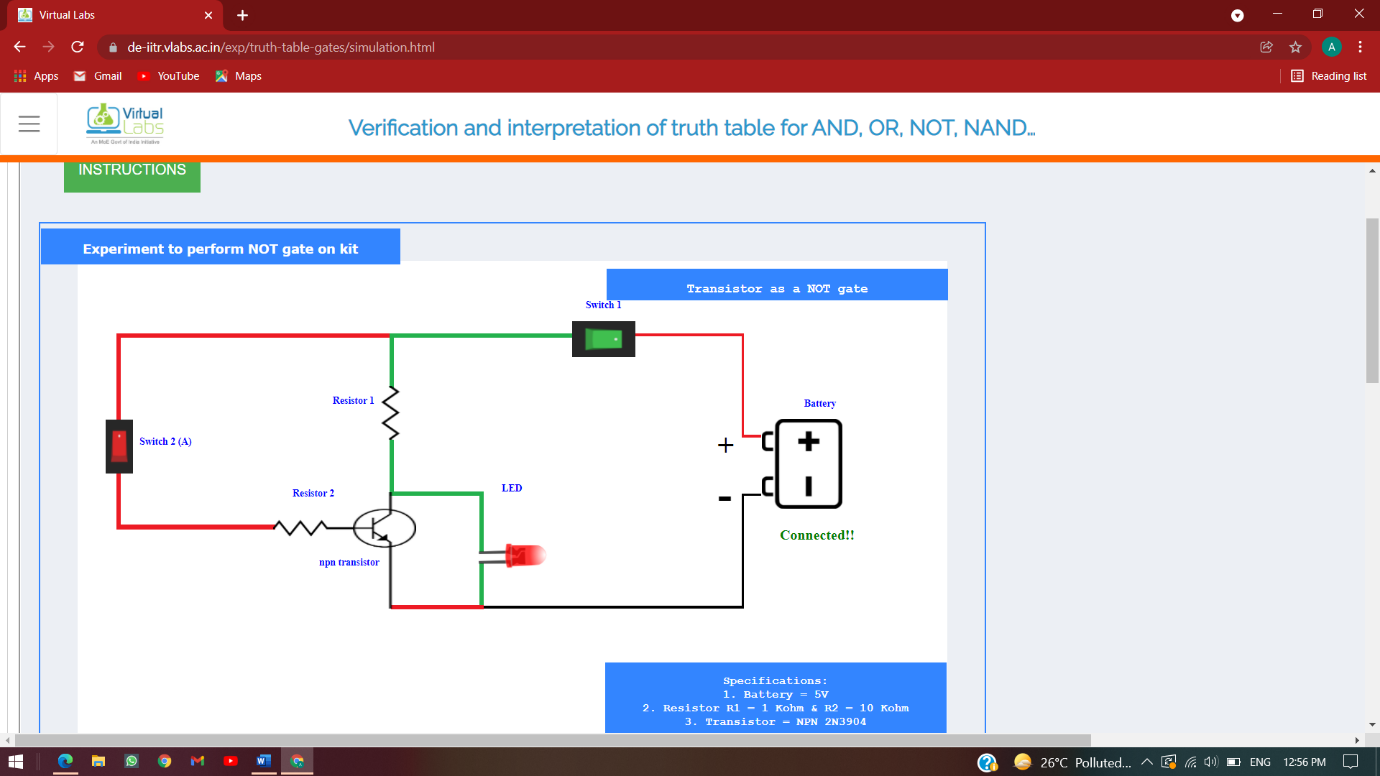
\includegraphics[width=0.9\linewidth]{img/exp3/4}
		\caption{}
		\label{fig:3:4}
	\end{figure}
		\begin{figure}[h]
		\centering
		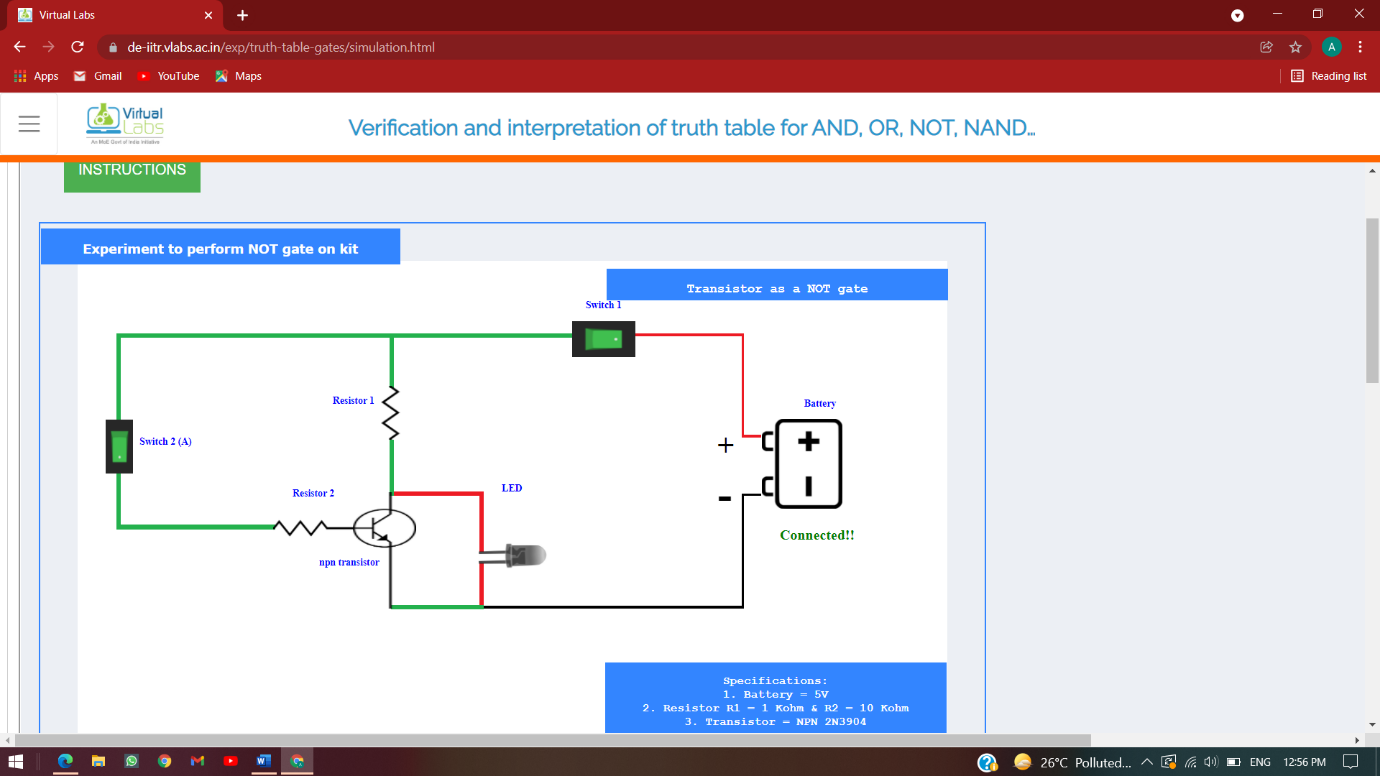
\includegraphics[width=0.9\linewidth]{img/exp3/5}
		\caption{}
		\label{fig:3:5}
	\end{figure}
		\begin{figure}[h]
		\centering
		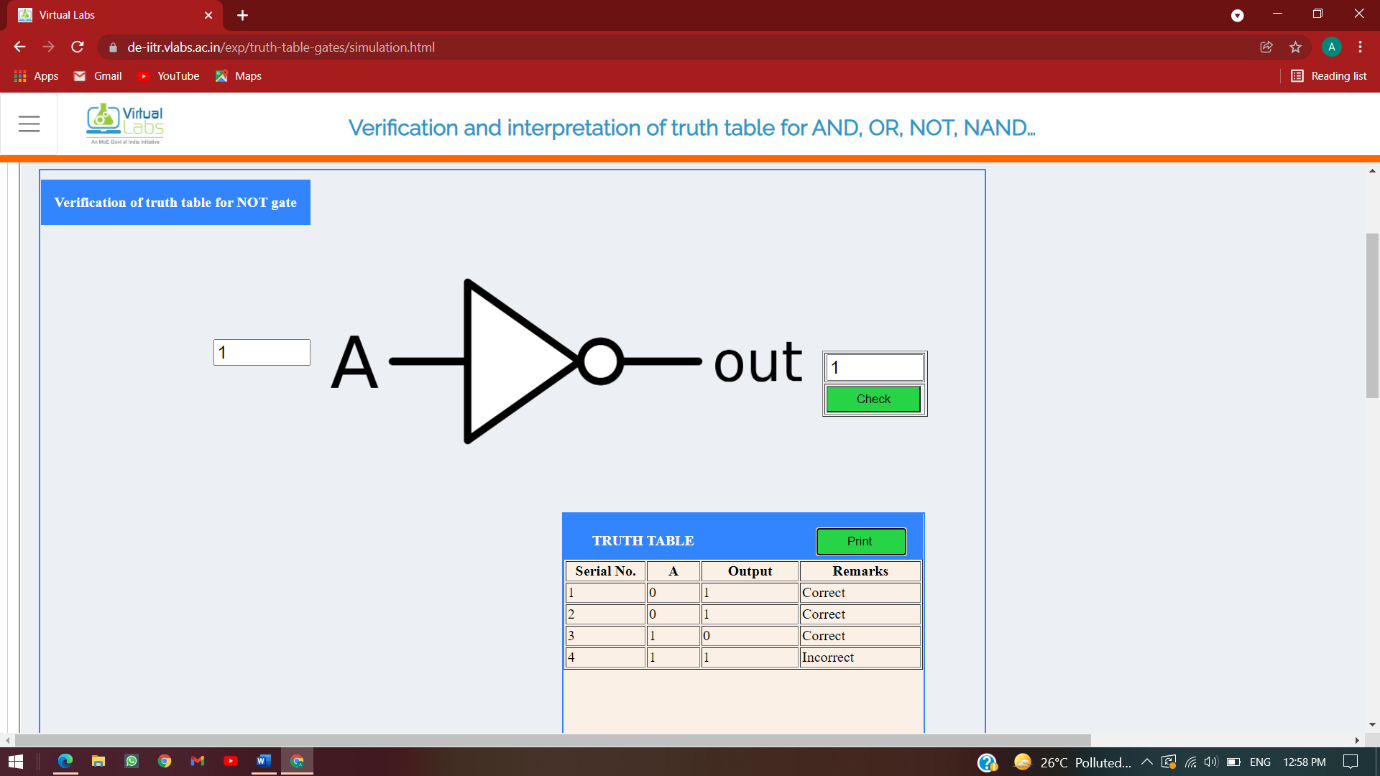
\includegraphics[width=0.9\linewidth]{img/exp3/6}
		\caption{}
		\label{fig:3:6}
	\end{figure}

\section{Conclusion}
As seen above , NOT gate negates the value of input . If the input is low , the output is higher and vice versa.

\section{Precautions}
	\begin{enumerate}
		\tightlist
		\item Make the connections when power supply is OFF.
		\item Ensure that the connections are tight.
		\item Change the status of inputs only when power supply is OFF.
	\end{enumerate}